\chapter{\textcolor{mycolor}{\textbf{Contexte général du projet et analyse des besoins}}}
\markboth{\chaptername\ \thechapter.\ Contexte général du projet et analyse des besoins}{}
\fancyhf{}
\fancyhead[L]{\small\itshape\nouppercase{\rightmark}}
\fancyfoot[L]{\small\itshape\nouppercase{\leftmark}}
\fancyfoot[R]{\small\itshape\thepage}
\renewcommand{\headrulewidth}{1pt}
\renewcommand{\footrulewidth}{0.4pt}

\vfill
\begin{flushright}{\Large\bfseries\textcolor{mycolor}{Introduction}}\end{flushright}
\addcontentsline{toc}{section}{Introduction}

Ce premier chapitre pose le cadre du projet. Nous présentons d'abord LIFEWISE, ses motivations, ses objectifs et
son scénario global. Nous exposons ensuite la problématique, puis le scénario pilote retenu pour cette année et son
périmètre. Nous analysons les besoins fonctionnels et non fonctionnels du système, avant de décrire l'organisation
de l'équipe et la planification du travail.

\clearpage

\section{Présentation générale du projet LIFEWISE}

\subsection{Contexte et motivations}

Les notifications, les tâches et les sollicitations numériques se multiplient, et l'organisation du quotidien en
devient plus difficile. La plupart des assistants personnels reposent pourtant sur des commandes explicites :
l'utilisateur formule une question, saisit un rappel ou consulte une application. Ils ne voient rien de la
situation réelle de la personne.

LIFEWISE propose un autre fonctionnement : un assistant qui prend en compte le contexte réel et fournit une alerte
ou une recommandation au moment où elle est utile. Pour y parvenir, le projet associe l'Internet des objets, la
vision par ordinateur, le traitement local des données et l'intelligence artificielle embarquée.

\subsection{Vision globale du système}

Un boîtier compact recueille des indices issus d'une caméra et de capteurs de mouvement, de porte et de luminosité.
Ces informations alimentent une chaîne logicielle qui décrit la situation observée, en extrait les éléments
pertinents, puis déclenche si nécessaire une assistance. Deux modèles d'intelligence artificielle se complètent :
un modèle vision-langage (VLM) transforme les images en descriptions structurées, et un petit modèle de langage
(SLM) croise ces descriptions avec les données des capteurs, des règles de fonctionnement et, si l'utilisateur y
consent, son historique.

Le dispositif a aussi une dimension analytique. Les événements et les recommandations sont enregistrés dans une base
locale SQLite. Un tableau de bord permet à l'utilisateur de consulter son historique, de corriger une observation
et de régler la fréquence des alertes.

La figure~\ref{fig:scenario-global} présente le scénario global imaginé dans le sujet : le même principe appliqué à
la maison, au travail et en déplacement.

\begin{figure}[H]
  \centering
  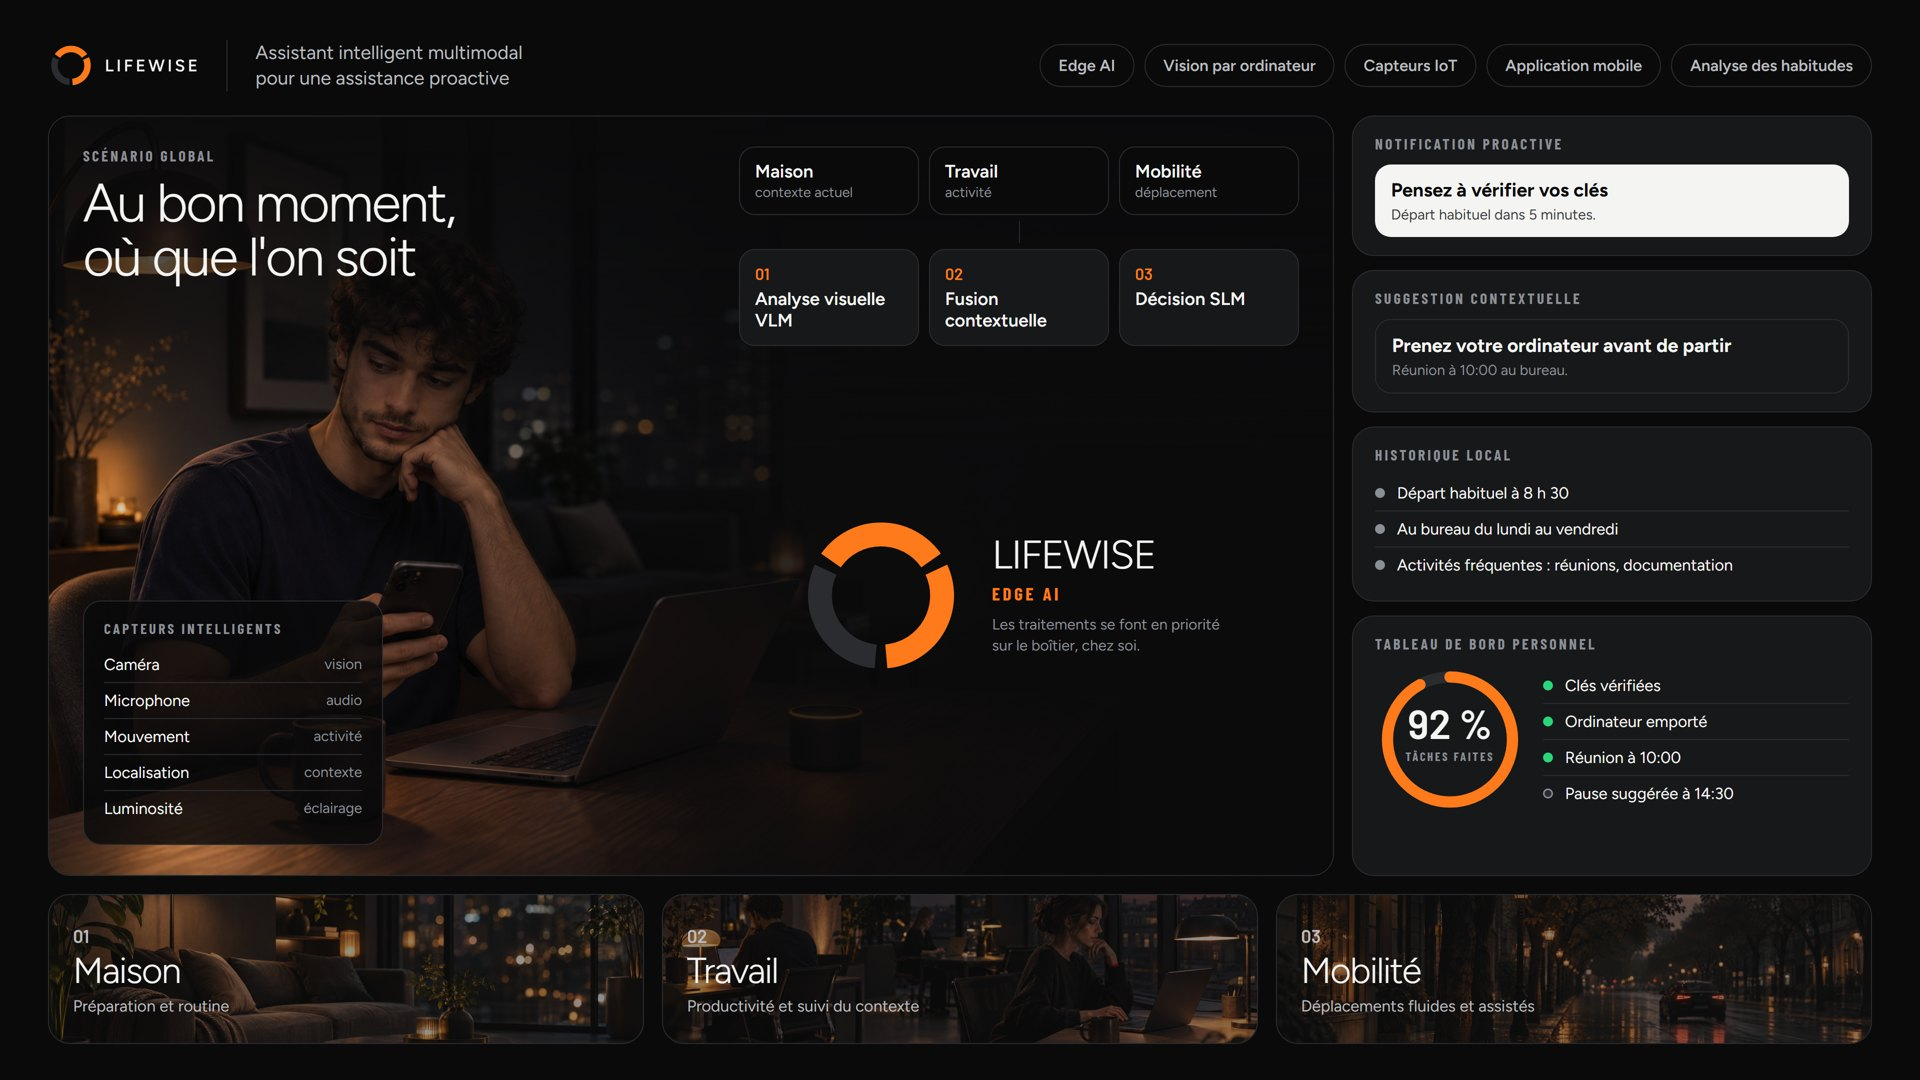
\includegraphics[width=\linewidth]{Figures/chapitre1/scenario-global.jpg}
  \caption{Scénario global de LIFEWISE : maison, travail et mobilité}
  \label{fig:scenario-global}
\end{figure}

\subsection{Objectifs du projet}

Le sujet fixe cinq objectifs stratégiques, résumés dans le tableau~\ref{tab:objectifs}.

\begin{table}[H]
  \centering
  \small
  \begin{tabularx}{\linewidth}{>{\bfseries}p{4.2cm}X}
    \toprule
    Objectif & Ce qu'il recouvre \\
    \midrule
    Assistance proactive & Détecter certaines situations d'oubli ou de désorganisation et proposer un rappel pertinent, validé par le contexte observé. \\
    Fusion des informations & Faire coopérer vision par ordinateur, capteurs IoT et historique local dans un pipeline multimodal structuré. \\
    Intelligence embarquée & Évaluer des modèles compacts, quantifiés si nécessaire, pour réduire la latence, la consommation et la dépendance à un service distant. \\
    Analyse des habitudes & Produire des synthèses et des recommandations fondées sur des observations explicables et contrôlables. \\
    Respect des données & Offrir une application simple et paramétrable, respectueuse du consentement, qui limite la conservation des données sensibles. \\
    \bottomrule
  \end{tabularx}
  \caption{Objectifs stratégiques du projet}
  \label{tab:objectifs}
\end{table}

\section{Problématique}

Trois difficultés se posent dès que l'on veut qu'un assistant agisse de lui-même.

La première est de \textbf{détecter la bonne situation}. Un assistant qui alerte trop souvent est vite désactivé ;
un assistant qui se tait au mauvais moment ne sert à rien. Il faut donc une situation définie avec précision, des
indices fiables et des règles qui limitent les déclenchements intempestifs.

La deuxième est de \textbf{ne pas conclure plus que ce qui est observé}. L'absence de clés sur une image prouve
seulement qu'elles n'ont pas été repérées dans le champ de la caméra. Elles peuvent être dans une poche. Le système
doit distinguer le fait observé de son interprétation, et formuler l'alerte comme une vérification : « Pensez à
vérifier vos clés ».

La troisième est de \textbf{tenir dans un petit appareil, en local}. Les modèles de vision et de langage sont
gourmands en mémoire et en calcul. Les faire tourner sur un Raspberry Pi oblige à choisir des modèles compacts, à
les quantifier si besoin et à mesurer précisément la latence obtenue.

À ces trois difficultés s'ajoute une contrainte de confiance : l'acquisition de données dans un environnement
personnel doit être encadrée. La conception prévoit l'activation explicite des capteurs, un indicateur de
fonctionnement, la possibilité de suspendre la collecte et la suppression de l'historique à la demande.

\section{Le projet pilote}

\subsection{Justification du choix}

Le scénario global ne peut pas être traité en entier dans le temps du projet. L'encadrant a fixé l'objectif :
réussir un scénario pilote de bout en bout. Nous avons retenu l'assistance à la sortie du domicile, que le sujet
présente comme premier scénario. Il a deux qualités : il est reproductible, et il mobilise toute la chaîne, des
capteurs jusqu'au téléphone.

\subsection{Description du scénario}

L'utilisateur se prépare à partir. Le système détecte le départ (ouverture de la porte, mouvement), cherche les
objets habituellement emportés (téléphone, clés, portefeuille), croise ces observations avec l'agenda (un
rendez-vous à 10~h, par exemple) et l'historique. Si le portefeuille n'est pas visible, le téléphone affiche :
« Pensez à vérifier votre portefeuille », avec deux choix, \textit{rappeler dans 5 minutes} ou \textit{ignorer}.
La réponse de l'utilisateur est inscrite dans l'historique local. La figure~\ref{fig:scenario-pilote} en présente
les étapes.

\begin{figure}[H]
  \centering
  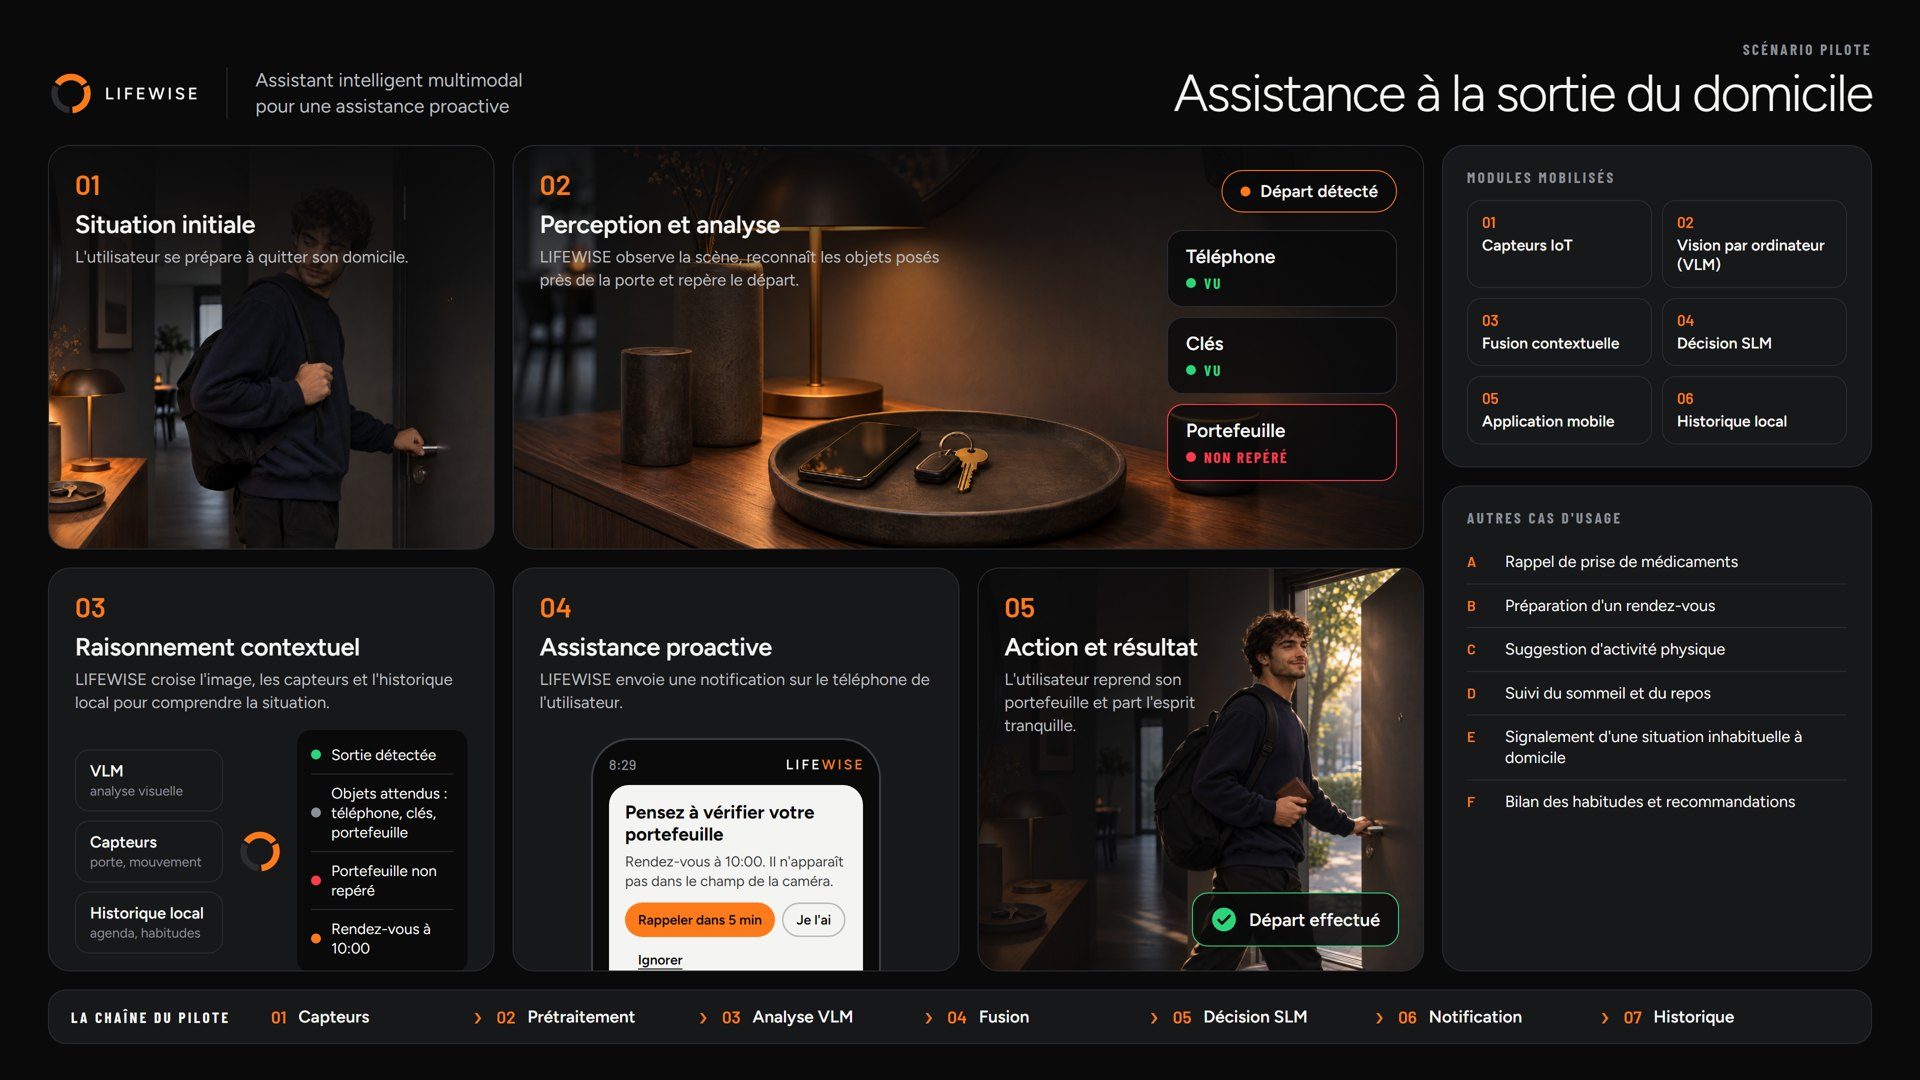
\includegraphics[width=\linewidth]{Figures/chapitre1/scenario-pilote.jpg}
  \caption{Scénario pilote : l'assistance à la sortie du domicile}
  \label{fig:scenario-pilote}
\end{figure}

\subsection{Fonctions retenues pour le prototype}

Le prototype doit réaliser la chaîne suivante, en sept étapes : acquisition par les capteurs, prétraitement,
analyse visuelle par le VLM, fusion contextuelle, décision par le SLM, notification sur le téléphone, et
inscription dans l'historique local.

\subsection{Limites du périmètre}

Le prototype ne traite ni le scénario au travail ni celui en déplacement. Le microphone, la centrale inertielle et
la localisation, cités par le sujet, ne sont pas utilisés : le scénario pilote n'en a pas besoin. Le dialogue avec
l'assistant (« Comment ai-je organisé mon temps cette semaine ? ») et l'export vers Power BI sont laissés aux
perspectives.

\section{Analyse des besoins}

\subsection{Acteurs}

Le système a un acteur principal, l'utilisateur, qui reçoit les alertes, y répond, consulte son historique et
règle l'assistant. L'équipe de développement intervient comme acteur secondaire pendant les essais : elle prépare
les scénarios, annote les données et mesure les performances.

\subsection{Besoins fonctionnels}

Le sujet découpe le système en six modules, chacun relié aux autres par une interface explicite. Le
tableau~\ref{tab:modules} résume ce que chacun doit faire.

\begin{table}[H]
  \centering
  \small
  \begin{tabularx}{\linewidth}{>{\bfseries}p{4.2cm}X}
    \toprule
    Module & Besoin \\
    \midrule
    1. Acquisition multimodale & Capter les images et les mesures (mouvement, porte, luminosité) et les horodater. \\
    2. Prétraitement et contexte & Filtrer et normaliser les données, sélectionner les images utiles, construire l'objet « contexte ». \\
    3. Compréhension visuelle (VLM) & Dire quels objets sont vus sur une image, avec un niveau de confiance. \\
    4. Fusion et décision (SLM) & Croiser les objets vus, les capteurs et l'agenda ; décider d'une action et la justifier. \\
    5. Application mobile & Afficher l'alerte, proposer \textit{rappeler dans 5 minutes} ou \textit{ignorer}, montrer l'historique, régler et suspendre la collecte. \\
    6. Historique et tableau de bord & Conserver les événements dans SQLite ; les afficher avec des indicateurs ; permettre la correction et la suppression. \\
    \bottomrule
  \end{tabularx}
  \caption{Besoins fonctionnels des six modules}
  \label{tab:modules}
\end{table}

\subsection{Besoins non fonctionnels}

\begin{itemize}
  \item \textbf{Exécution locale} : les images ne quittent pas l'appareil ; les modèles tournent sur le Raspberry Pi ou sur un ordinateur de la maison.
  \item \textbf{Latence} : l'alerte doit arriver pendant que l'utilisateur est encore à la porte.
  \item \textbf{Fiabilité} : peu de fausses alertes, et aucune alerte sans départ détecté.
  \item \textbf{Explicabilité} : chaque décision est accompagnée d'une justification courte.
  \item \textbf{Contrôle par l'utilisateur} : activation explicite, suspension, réglage de la fréquence, suppression de l'historique.
\end{itemize}

\subsection{Indicateurs de performance}

Le sujet définit sept dimensions d'évaluation (tableau~\ref{tab:kpi}). Les seuils de réussite seront fixés après
les premiers essais, en fonction du matériel et des jeux de test.

\begin{table}[H]
  \centering
  \small
  \begin{tabularx}{\linewidth}{>{\bfseries}p{4.2cm}X}
    \toprule
    Dimension & Mesure envisagée \\
    \midrule
    Perception multimodale & Journal structuré des événements, disponibilité des capteurs \\
    Analyse visuelle & Objets bien vus, manqués et inventés sur des scénarios annotés \\
    Raisonnement & Taux de décisions correctes, fausses alertes, motifs de décision \\
    Assistance proactive & Latence mesurée, taux d'alertes jugées utiles \\
    Analyse historique & Indicateurs et graphiques consultables par l'utilisateur \\
    Expérience utilisateur & Tests d'usage : accès à l'historique, suppression, réglages \\
    Faisabilité Edge AI & Processeur, mémoire et temps de traitement sur le matériel retenu \\
    \bottomrule
  \end{tabularx}
  \caption{Indicateurs de performance du projet}
  \label{tab:kpi}
\end{table}

\subsection{Contraintes matérielles et logicielles}

Le matériel est fourni par l'encadrant : un Raspberry Pi, une caméra à choisir et des capteurs. Le Raspberry Pi
sert de banc d'essai pour l'Edge AI ; il ne bloque pas le reste du travail, car la chaîne accepte aussi les images
de la caméra d'un téléphone ou d'une webcam. Côté logiciel, Python est l'environnement principal, avec OpenCV,
Pandas, PyTorch, l'écosystème Hugging Face et SQLite.

\subsection{Protection des données}

Les personnes présentes dans le champ des capteurs pendant les essais en sont informées, et les scénarios sont
réalisés dans des lieux autorisés. Aucune photo où l'on reconnaît une personne n'est déposée dans le dépôt du
projet. Les images brutes suivent une politique de conservation distincte, plus courte que celle des événements.

\section{Organisation et planification du projet}

\subsection{Méthodologie de travail}

Nous avons découpé le travail selon la chaîne elle-même : une sous-équipe par maillon. Chacune sait ce qu'elle
reçoit, ce qu'elle produit et à qui elle le transmet. Les échanges passent par un contrat d'interface au format
JSON, écrit en première semaine par la sous-équipe Data avec un représentant de chaque sous-équipe. Chaque maillon
est d'abord prouvé sur des données simulées, avant d'être branché sur la chaîne réelle.

\subsection{Les six sous-équipes}

Le tableau~\ref{tab:equipes} présente la composition des sous-équipes. Karamo Sylla et Adila Yassir sont les
responsables du projet.

\begin{table}[H]
  \centering
  \small
  \begin{tabularx}{\linewidth}{>{\bfseries}p{4.2cm}Xp{2cm}}
    \toprule
    Sous-équipe & Membres & Référent \\
    \midrule
    1. IoT et matériel & Adila Yassir, Abrini Mohamed, Mohamed Channa & Adila \\
    2. Data & Michel Sagesse Kolie, Zakaria Tahiri, Amine Sbah & Michel \\
    3. Vision (VLM) & Bachirou Konate, Yasser Nadi & Bachirou \\
    4. Décision et backend & Adnane Qassiri, Aymane Azaagag & Adnane \\
    5. Application web & Saïd Jadli, Aymane Hayoun & Saïd \\
    6. Application mobile et coordination & Karamo Sylla & Karamo \\
    \bottomrule
  \end{tabularx}
  \caption{Composition des sous-équipes}
  \label{tab:equipes}
\end{table}

\subsection{Répartition des responsabilités}

\begin{table}[H]
  \centering
  \small
  \begin{tabularx}{\linewidth}{>{\bfseries}p{4.2cm}X}
    \toprule
    Sous-équipe & Mission \\
    \midrule
    1. IoT et matériel & Monter le banc d'essai : Raspberry Pi, caméra et capteurs qui produisent des mesures et des images horodatées. \\
    2. Data & Écrire le contrat d'interface, préparer les données, constituer les scénarios annotés, concevoir la base SQLite. \\
    3. Vision (VLM) & Comparer Moondream2, LLaVA et un détecteur léger ; dire quels objets sont vus et avec quelle confiance. \\
    4. Décision et backend & Écrire les règles, produire la décision avec un SLM, enchaîner les modules, exposer l'API des applications. \\
    5. Application web & Réaliser le tableau de bord : historique, indicateurs, réglages, accès en ligne au projet. \\
    6. Application mobile et coordination & Réaliser l'application mobile, intégrer la chaîne, assembler le rapport et le guide. \\
    \bottomrule
  \end{tabularx}
  \caption{Missions des sous-équipes}
  \label{tab:missions}
\end{table}

Le détail des tâches, des livrables et des échéances de chaque sous-équipe figure en annexe~A.

\subsection{Outils de gestion et de collaboration}

Le code vit dans un dépôt GitHub commun (\url{https://github.com/Kaaramo/lifewise}), avec un dossier par
sous-équipe et une branche par membre. Une modification rejoint la branche principale par une demande de fusion,
relue par le référent de la sous-équipe. Ce rapport est rédigé en LaTeX dans le même dépôt : chaque sous-équipe
écrit ses sections dans son dossier, et la coordination les assemble. Un guide de présentation, tenu à jour à
chaque remise, complète le dispositif.

\subsection{Planification}

Le sujet prévoyait quatre mois. Nous en gardons la logique, logiciel sur données simulées d'abord et matériel en
parallèle, sur cinq semaines de développement (figure~\ref{fig:gantt}). Les dates sont proposées dans l'attente
de la date de rendu fixée par l'encadrant.

\begin{figure}[H]
  \centering
  \small
  \begin{ganttchart}[
      x unit=1.35cm, y unit title=0.6cm, y unit chart=0.55cm,
      vgrid, hgrid,
      title label font=\footnotesize\bfseries,
      bar label font=\footnotesize,
      bar/.append style={fill=mycolor!70, draw=mycolor},
      bar height=0.55
    ]{1}{6}
    \gantttitle{Avant S1}{1} \gantttitle{S1}{1} \gantttitle{S2}{1} \gantttitle{S3}{1} \gantttitle{S4}{1} \gantttitle{Fin}{1} \\
    \ganttbar{Équipes, dépôt, environnement}{1}{1} \\
    \ganttbar{Contrat d'interface, scénarios}{2}{2} \\
    \ganttbar{Matériel, choix de la caméra}{2}{3} \\
    \ganttbar{Essais VLM et SLM}{2}{3} \\
    \ganttbar{Chaîne sur ordinateur}{3}{3} \\
    \ganttbar{Chaîne sur Raspberry Pi}{4}{4} \\
    \ganttbar{Applications reliées}{3}{4} \\
    \ganttbar{Démonstration et mesures}{5}{5} \\
    \ganttbar{Rapport et guide finaux}{6}{6}
  \end{ganttchart}
  \caption{Diagramme de Gantt du projet}
  \label{fig:gantt}
\end{figure}

\section*{Conclusion}
\addcontentsline{toc}{section}{Conclusion}

Ce chapitre a posé le cadre du projet : un assistant qui agit de lui-même, testé sur un scénario précis, la sortie
du domicile, et construit par six sous-équipes autour d'une chaîne en sept étapes. Le chapitre suivant présente
l'état de l'art des technologies sur lesquelles repose cette chaîne.
